\section{Attacco con ricerca non lineare}

Un alternativa ai confronti lineari può essere quella di usare strutture dati che fanno uso in qualche modo dell'hashing per indirizzare correttamente le stringhe. Nel caso più semplice , si può usare una hashmap, in cui si possono allocare le stringhe del database intepretando gli hash SHA256 come numeri Big Int e poi sfruttando l'aritmetica modulare si possono posizionare a opportuni indirizzi di questa struttura. Una volta effettuata questa operazione si può eseguire l'hashing delle password da cercare e individuare con lo stesso procedimento se questo è contenuto o meno nella hashmap. 

\subsection{Un semplice caso sequenziale}
Il caso sequenziale a singolo nodo, implementa in modo molto semplice i passi descritti precedentemente, un possibile pseudocodice 

\begin{lstlisting}
    const space = I in (0,inf) // decide at compile time the size of the array hashmap
    database = load_database()
    password = load_password()
    map = hashmap(space)
    for i in 0..database.len do{
        index = bigint_read(hash) % space 
        map.append(index,{database[i].user,database[i].hash})
    }
    for pw in password do{
        pwhash = hash(pw)
        index = bigint_read(pwhash)%space 
        if map.contains(pwhash,index){
            notify_password(pw)
        }
    }
\end{lstlisting}

Per valutare le prestazioni di questa soluzione bisogna cambiare la funzione comparazione $C(X,Y)$ , che considerava di scorrere tutta la lista di hash del database per trovare un hash corrispondente. Infatti una hashmap nel caso migliore permetterebbe un accesso diretto al contenuto, di fatto quando le chiavi sono così tante un certo quantitativo di collisioni è inevitabile, per fortuna si può stimare il numero di collisioni atteso a seconda di quanti spazi sono presenti nella mappa e quanti chiavi saranno aggiunte:
$E[O]=K-H_s +H_s *(\frac{H_s -1 }{H_s})^{K}$ dove $H_s$ sono gli spazi disponibili nella hashmap. Da qui si può ricavare un modello che stimi correttamente il tempo di esecuzione totale  
$$
T_{seq}= C_h(N,K,H_s)+ H(K) + L(K) + L(N) + I(N) + I(K)
$$
dove:
\begin{itemize}
    \item $C_h(N,K,H_s)=$: è il tempo impiegato dalla funzione di comparazione considerando gli slot disponibili della hashmap $H_s$
    \item $I(X)$ : è il tempo impiegato per trasformare un hash in un big int e calcolarne il modulo, seguendo il processo fatto per la funzione di hashing, si è visto che il tempo massimo è di 8 us
\end{itemize}
 In questa casistica vale la pena pensare allo spazio che si stima venga occupato, poichè è richiesto che tutto il database venga in qualche modo caricato in memoria a differenza dei casi precedenti, dove invece è possibile ad esempio creare uno stream continuo tra lo storage e i nodi in modo da dover caricare solo porzioni più piccole di questi file così grandi. Questa funzione che rappresenta lo spazio occupato si può scrivere come  
$M_{seq}=N*SHA_{size}+K*SHA_{size}+H_s*8$, dove $SHA_{size}$ è la quantità di byte necessaria per memorizzare un singolo hash nell'algoritmo scelto, nel caso di SHA256 è 32 byte, $H_s$ è la dimensione della hashmap che va moltiplicata per la dimensione di un puntatore , nel caso di un architettura a 64 bit è 8 byte. Ad esempio se si volesse eseguire il test su un database con $10^6$ chiavi contro un file di 10000 chiavi, usando una hashmap grande il doppio del database , si occuperebbe uno spazio di 
$M=10^6*32+10^4*32+2* 10^6*8\approx46.6_{MB}$  che è uno spazio del tutto gestibile da un qualunque computer moderno, ma si evince bene già subito che non appena si sale di anche solo un ordine di grandezza la quantità di dati cresce significativamente. 

\subsection{Attacco con HashMap distribuita}
Parallelizzare un attacco del genere non è immediato, neanche sfruttando un architettura main worker. Tuttavia un primo metodo piuttosto semplice può prendere liberamente ispirazione a un utilizzo abbastanza popolare di una struttura come una hash table, una hash table distribuita. Oggi questa struttura alimenta il protocollo Torrent per trasferire file in p2p, le DHT possono essere statiche o dinamiche, in questo ci si può servire della prima tipologia , poichè normalmente il numero di nodi che partecipano al calcolo è fisso in un architettura HPC.

Per usare una DHT l'approccio prevede sempre un architettura main worker, ogni worker istanzia in memoria una normale hash table. Il main legge il file del database e calcola il modulo dell'hash a seconda di quanti nodi ci sono in rete, poi manda al nodo indicato dal risultato l'hash se è diverso da se stesso, altrimenti lo memorizza. Successivamente il nodo root scorre il file delle password ed effettua lo stesso processo con ogni entry e se lui o un altro nodo trovano una corrispondenza lo notificano , in pseudocodice

\begin{lstlisting}

    rank = world().rank 
    if rank is root{
        map = hashmap(size)
        password = load_password()
        database = load_database()
        for entry in database do{
            dest = big_int(hash) % world().size
            if dest is not root{
                send(hash,dest,database_tag)
            }
            else{
                index = big_int(hash) % size
                map.insert(index,entry.user,entry.hash)
            }
        }
        for pw in password do {
            pwhash = hash(pw)
            dest = big_int(pwhash) % world.size()
            if dest is not root{
            send(pw,dest,pw_tag)
            }
            else{
                entry = map[pwhash]
                if entry != null{
                    notify_password(pw,entry.user,entry.hash)
                }
            }
        }
    }
    else{
        map = hashmap(size)
        message = recv(root)
        if message.tag is database_tag{
            index = big_int(message.hash)%size
            map.insert(message.hash,index)
        }
        else {
            pw = message.pw 
            hashpw = hash(pw)
            entry = map[hashpw]
            if entry != null{
                notify_password(pw,entry.user,entry.hash)
            }
        }
    }
\end{lstlisting}

Per ricavare le misure di performance si possono usare tutte le variabili del caso precedente, per cui si può scrivere
$$
T_{comp}= C_h(N,K,H_s*P) +  H(K)  + I(N)*P + I(P)
$$

Il vantaggio sostanziale per cui è che si abbassa notelvolmente la probabilità di collisioni nelle hashmap, di contro si aggiunge un overhead dovuto alla comunicazione, che però è ottimizzata poichè si conosce già il nodo possibile detentore di una certa password.
$$
T_{comm} =  L(K) + L(N) + S(N)+S(K)
$$

Tuttavia i risultati della simulazione mostrano uno scarso rendimento rispetto alla prima delle soluzioni parallele in cui si cercavano gli hash corrispondenti utilizzando un approccio di ricerca lineare. 

\begin{figure}[H]
    \centering
    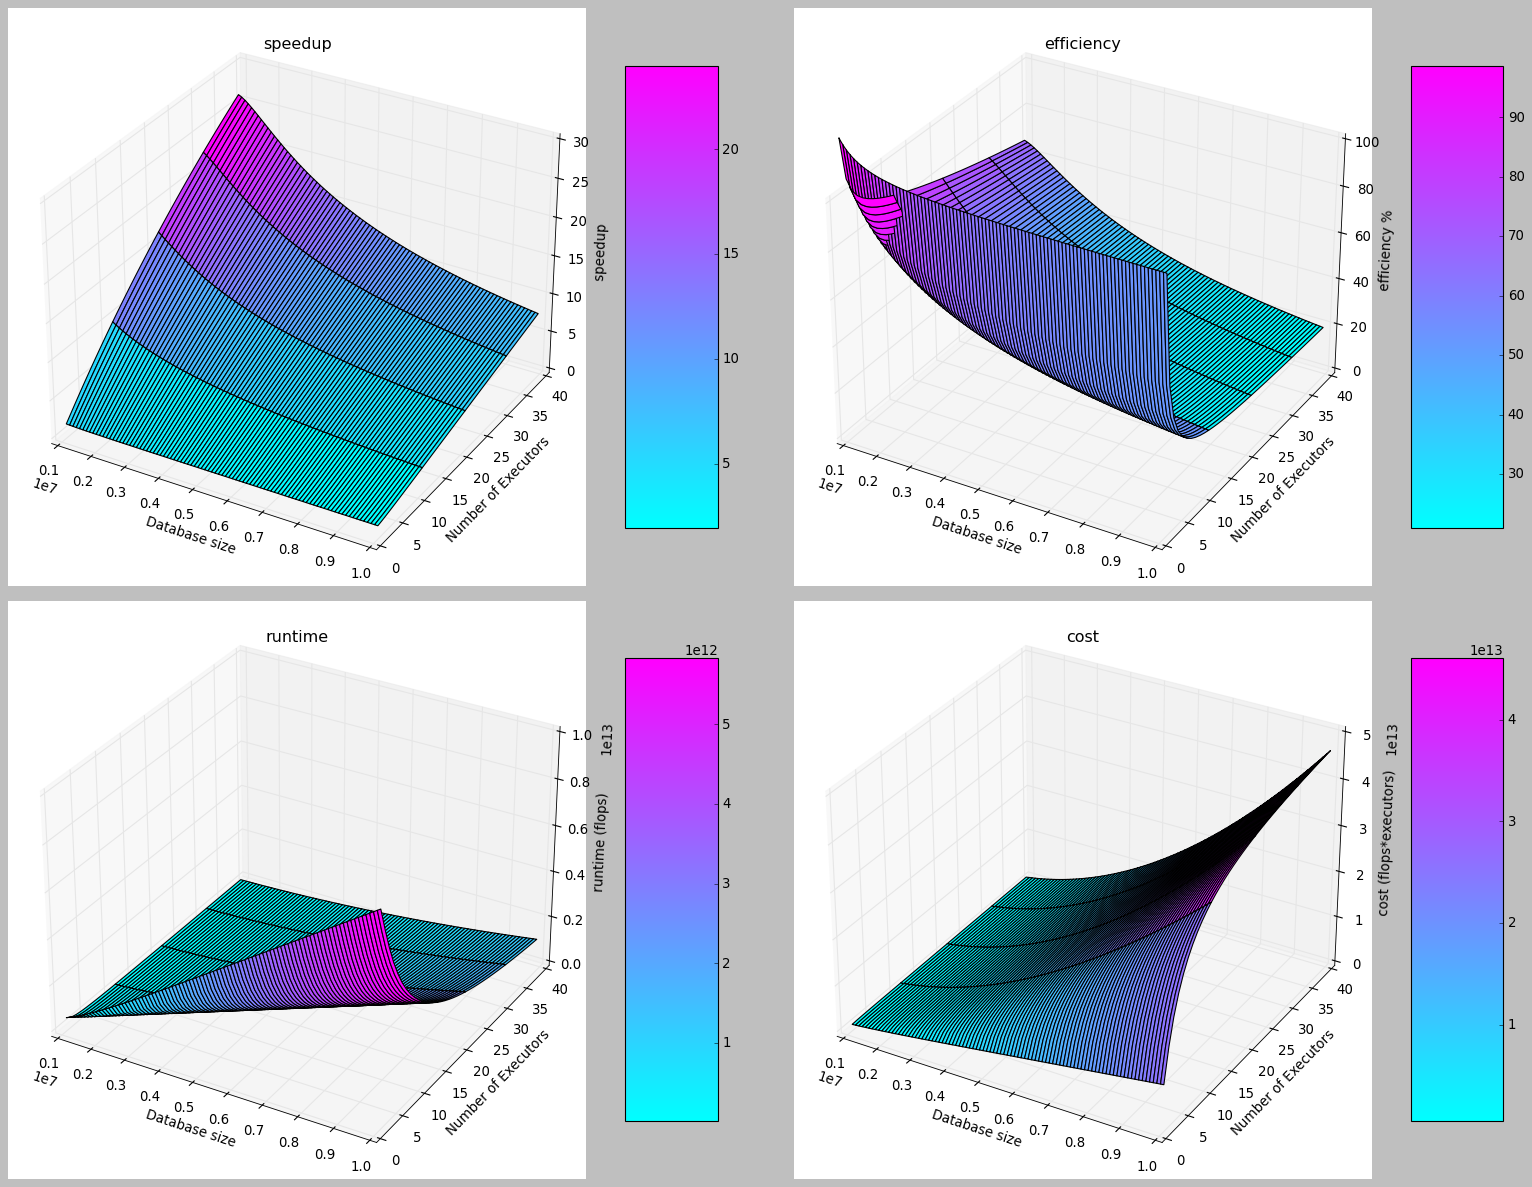
\includegraphics[width=0.9\textwidth]{images/mainworkerhashmap.png}
    \caption{Misure ottenute dalla simulazione sul caso della hashmap distribuita}
\end{figure}

\section{Conclusioni}
Da una prima comparazione parrebbe chiaro che il metodo che più scala con la presenza di esecutori sia l'archittettura ad anello con 
task dinamici, di lunghezza fissa. 
\begin{figure}[H]
    \centering
    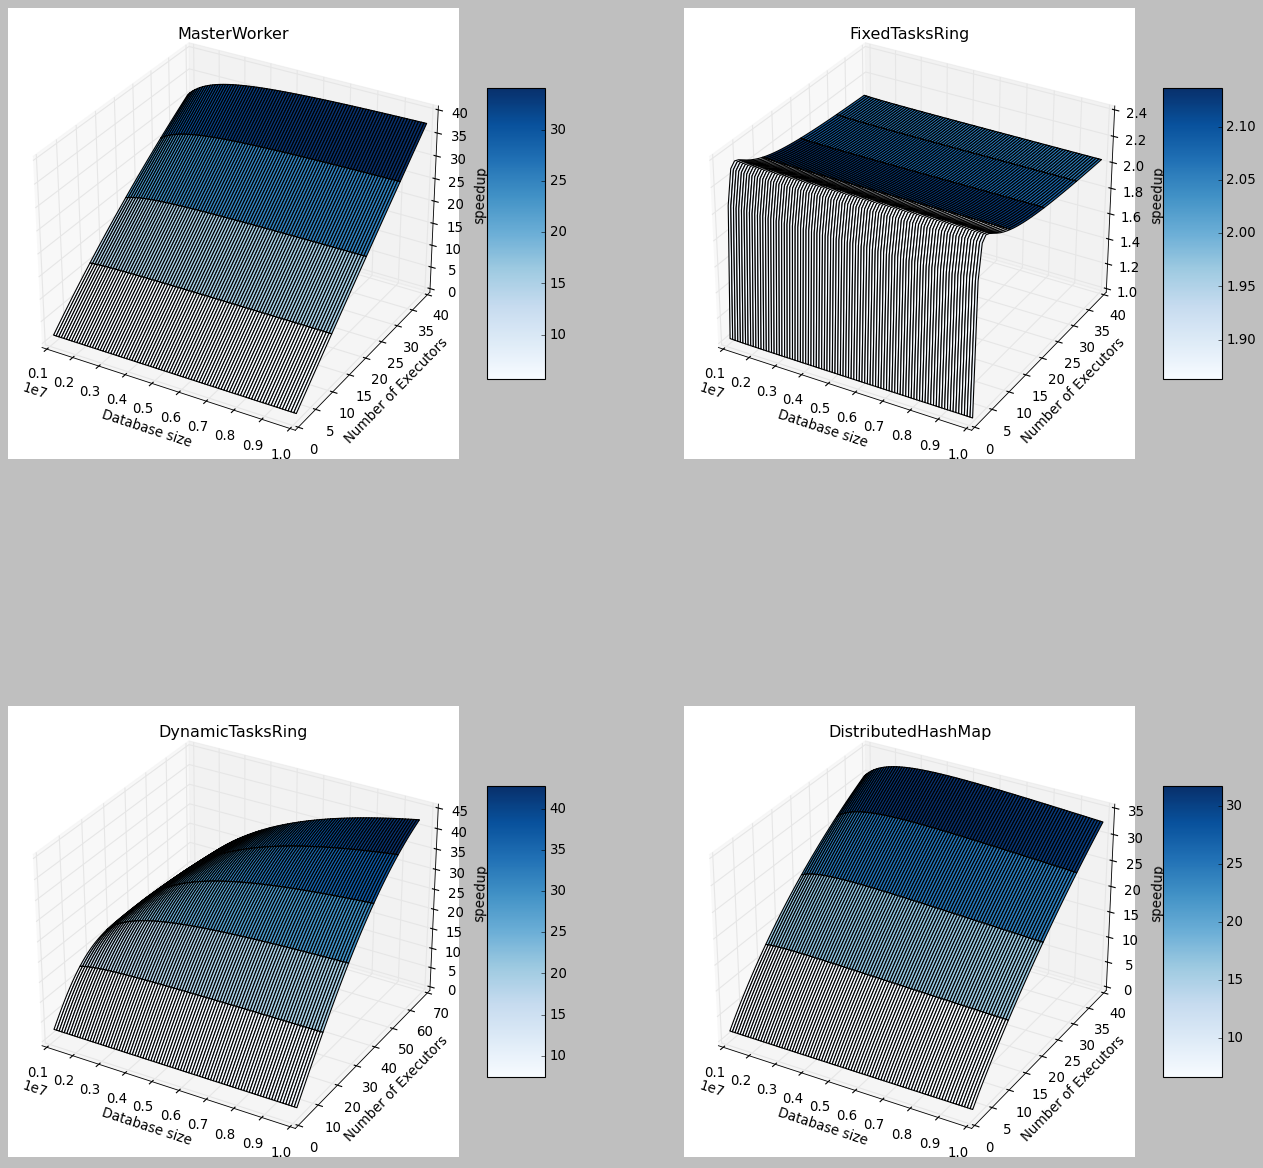
\includegraphics[width=0.9\textwidth]{images/confrontation.png}
    \caption{Comparazione degli speedup}
\end{figure}

Tuttavia sembra essere meno efficiente, man mano che che vengono aggiunti gli esecutori, del più banale master worker. 

\begin{figure}[H]
    \centering
    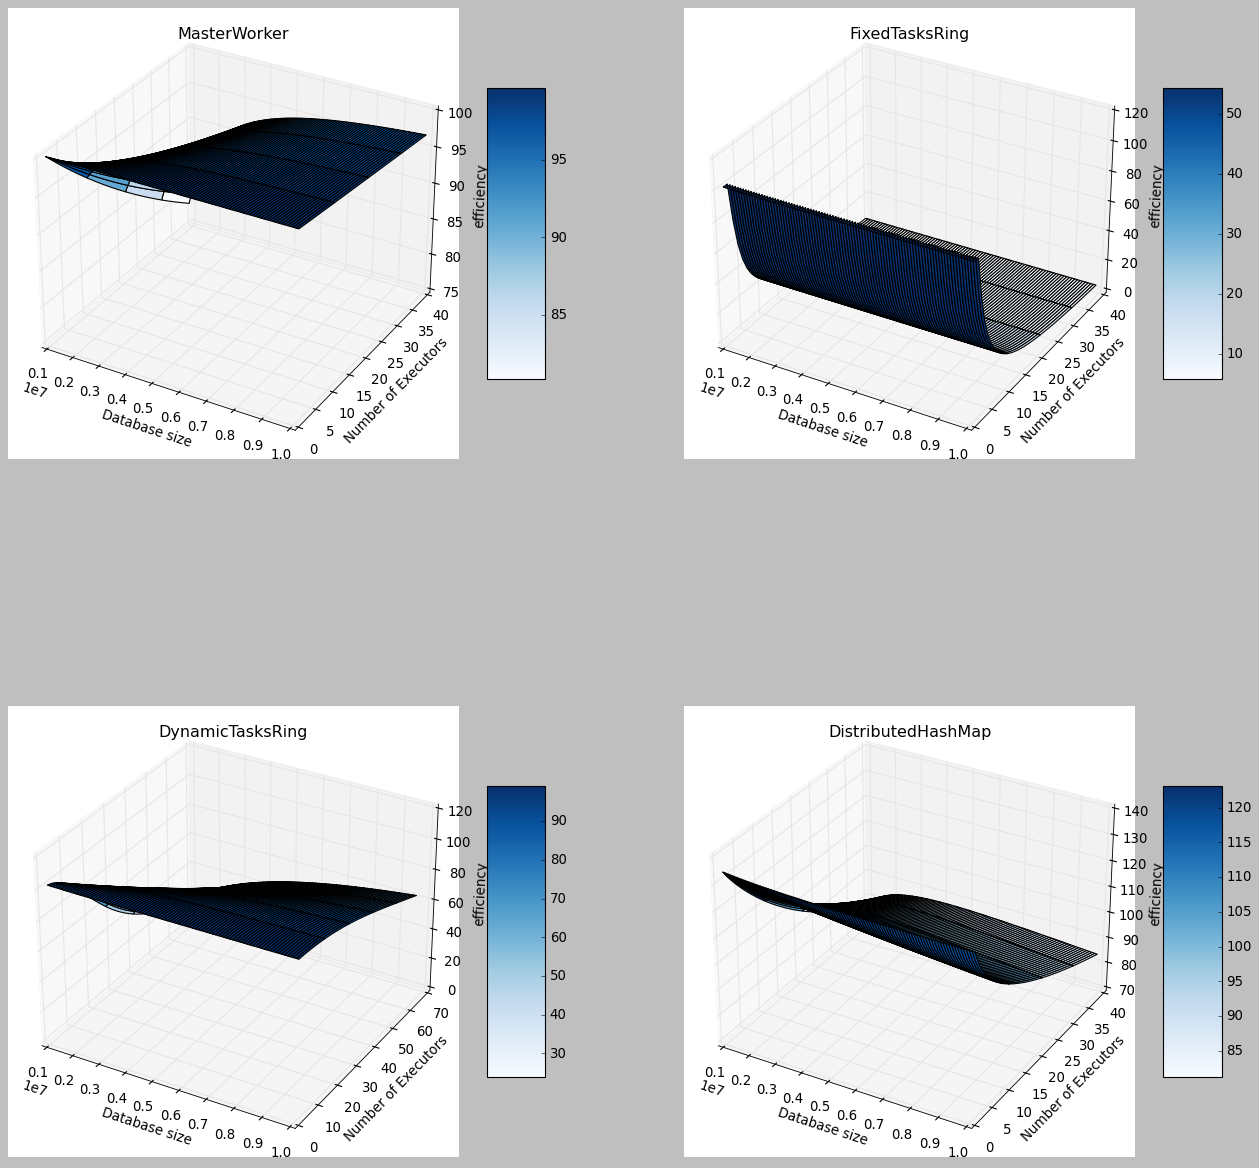
\includegraphics[width=0.9\textwidth]{images/efficiency_comparison.png}
    \caption{Comparazione delle efficienze}
\end{figure}

Nonostante le differenze architetturali comunque, tutte le architetture performano piuttosto bene a livello teorico, meno che quella ad anello con numero di task fissi, che è l'unica che si può scartare a priori. Al di là delle performance, tutte e 3 le architetture hanno motivi diversi per essere implementate, la prima che è la più semplice è particolarmente facile e veloce da applicare, oltretutto funziona anche piuttosto bene anche in contesti non distribuiti, ad esempio in multithread sulla stessa macchina o su una GPU. L'architettura ad anello invece, come già accennato, è efficace in un contesto in cui si vuole trattare il database come un flusso. Invece la DHT può risultare efficace se si hanno molti dispositivi, magari con poca capacità di calcolo ma molta memoria, da cui trarrebbero più beneficio rispetto che usando le altre due architetture. Non esiste quindi un architettura che a livello teorico superi in tutto e per tutto le altre, l'unico modo per capire quale sia la migliore per l'hardware che si ha a disposizione è quella di eseguire un benchmark.